\documentclass[landscape]{slides}
\usepackage{amsmath}
\usepackage{amssymb}
\usepackage{amstext}
\usepackage{enumerate}
\usepackage{epsfig}
\usepackage{graphics}
\usepackage{ifthen}
\usepackage[latin1]{inputenc}
\usepackage{listings}
\usepackage{mathpartir}
\usepackage{mathrsfs}
\usepackage{moreverb}
\usepackage{stmaryrd}
\usepackage{textcomp}
\usepackage{times}
\usepackage{url}

%
% For landscape mode slides:
%  1) use \documentclass[landscape]{slides}
%  2) latex main
%  2) dvips -tlandscape main -o 
%
% You can also try
%  1) use \documentclass[landscape]{slides}
%  2) latex main
%  3) texdvipdfm -l main.dvi
%
\usepackage{graphics}
\usepackage{color}
\usepackage{epsfig}
%\setlength{\oddsidemargin}{-30pt}
%\setlength{\evensidemargin}{-30pt}
\setlength{\topmargin}{-0.75in}
\setlength{\textheight}{7in}
% colour defs
\input colordvi
\definecolor{headcolor}{rgb}{0.55,0,0}
%\definecolor{itemcolor}{rgb}{0.1,0.1,0.55}
%\definecolor{itemcolor}{named}{SkyBlue}
%\definecolor{tickmarkcolor}{rgb}{0.5,0.1,0.5}
%\definecolor{tickmarkcolor}{named}{SkyBlue}
%\definecolor{titlecolor}{rgb}{0.65,0.1,0.1}
% \definecolor{titlecolor}{rgb}{0.7,0.5,0.9}
% \definecolor{tickmarkcolor}{rgb}{0.7,0.5,0.9}
% \definecolor{emphcolor}{rgb}{0.7,0.5,0.9}
%\definecolor{titlecolor}{rgb}{0.8,0.7,0.2}
%\definecolor{tickmarkcolor}{rgb}{0.85,0.84,0.1}
\definecolor{titlecolor}{cmyk}{0.98,.3,0,0.43}
\definecolor{tickmarkcolor}{cmyk}{0.98,.3,0,0.43}
%\definecolor{emphcolor}{rgb}{1.0,0.6,0.3}
\definecolor{emphcolor}{named}{BrickRed}
\definecolor{refcolor}{rgb}{0.,.4,.4}
%\def\Red#1{\Color{0 0.70 0.70 0.2}{#1}}
%\def\Green#1{\Color{0.70 0 0.5 0.2}{#1}}
%\def\Blue#1{\Color{0.70 0 0 0.2}{#1}}
\definecolor{Beige}   {rgb}{0.96,0.96,0.86}
%\definecolor{Background}   {rgb}{.97,.94,0.82}
\definecolor{Background}   {rgb}{1.,1.,1.}
\definecolor{MyYellow}{rgb}{1.,0.84,0.8}
\definecolor{Gold}  {rgb}{1.0,0.84,0.}
\definecolor{White} {named}{White}
%\definecolor{DarkGold}  {rgb}{.5,0.42,0.}
\definecolor{DarkGold}  {rgb}{.3,0.28,0.}
\definecolor{Blue}{rgb}{0.,0.,1.}
\definecolor{Pink}{rgb}{1.,0.75,0.8}
\definecolor{light-blue}{rgb}{0.8,0.85,1}
\definecolor{mygrey}{gray}{0.75}
\definecolor{darkgrey}{gray}{0.40}
\definecolor{greenyellow}{named}{GreenYellow}
\definecolor{myblack}{named}{Black}
% existing color names:
%GreenYellow, Yellow, Goldenrod, Dandelion, Apricot, Peach, Melon,
%YellowOrange, Orange, BurntOrange, Bittersweet, RedOrange, Mahogany,
%Maroon, BrickRed, Red, OrangeRed, RubineRed, WildStrawberry, Salmon,
%CarnationPink, Magenta, VioletRed, Rhodamine, Mulberry, RedViolet,
%Fuchsia, Lavender, Thistle, Orchid, DarkOrchid, Purple, Plum, Violet,
%RoyalPurple, BlueViolet, Periwinkle, CadetBlue, CornflowerBlue,
%MidnightBlue, NavyBlue, RoyalBlue, Blue, Cerulean, Cyan, ProcessBlue,
%SkyBlue, Turquoise, TealBlue, Aquamarine, BlueGreen, Emerald,
%JungleGreen, SeaGreen, Green, ForestGreen, PineGreen, LimeGreen,
%YellowGreen, SpringGreen, OliveGreen, RawSienna, Sepia, Brown, Tan,
%Gray, Black, White.

% new tick marks for itemize
\renewcommand{\labelitemi}{ {\color{tickmarkcolor}$\bullet$} }

% new tick marks for itemize
\renewcommand{\labelenumi}{
        {\color{tickmarkcolor} \arabic{enumi}}
}


% color versions of itemize/enumerate with less spacing
\newenvironment{citemize}{
        \vspace{-0.2in}
        \begin{itemize}
        \itemsep 0in
        %\color{itemcolor}
}{
        \end{itemize}
}
\newenvironment{cenumerate}{
        \vspace{-0.2in}
        \begin{enumerate}[\hspace{5mm}1.]
        \itemsep 0in
        %\color{itemcolor}
}{
        \end{enumerate}
}

% headed slide takes 1 parameter: the heading of the slide, which will
% appear at the topright of the page
\newenvironment{hslide}[1]{
        \begin{slide}
        \begin{flushright}
                {\color{headcolor} \tiny #1}
        \end{flushright}
}{
        \end{slide}
}

% titled slide takes 1 parameter: the heading of the slide, which will
% appear at the topright of the page
\newenvironment{tslide}[1]{
        \begin{slide}
        \begin{flushleft}
                {\bf \color{headcolor} #1}
        \end{flushleft}
}{
        \end{slide}
}

% title - displayed as emphasised
\newcommand{\stitle}[1]{
        { \bf \color{titlecolor} #1 }
}

% comments
\newcommand{\mknote}[1]{
        \begin{note}
                \begin{flushright}
                        {\it NOTES}
                \end{flushright}
                {\scriptsize #1
                
                end}
        \end{note}
}

% end web borrowed macros

\def\cemph#1{{\color{emphcolor}\emph{#1}}}
\def\ucemph#1{{\color{emphcolor}#1}}
\def\cref#1{{\color{refcolor}\small\emph{#1}}}
\def\bigref#1{{\color{refcolor}\emph{#1}}}
\def\cdesc#1{{\color{titlecolor}\small\emph{#1}}}
%\usepackage{times}
%\usepackage{mathptmx}
% beat slides class fonts into submission
% first, use most of package times
\renewcommand{\sfdefault}{phv}
\renewcommand{\rmdefault}{ptm}
\renewcommand{\ttdefault}{pcr}
% then, use most of package mathptm
\DeclareSymbolFont{operators}   {OT1}{ptmcm}{m}{n}
\DeclareSymbolFont{letters}     {OML}{ptmcm}{m}{it}
\DeclareSymbolFont{symbols}     {OMS}{pzccm}{m}{n}
\DeclareSymbolFont{largesymbols}{OMX}{psycm}{m}{n}
\DeclareSymbolFont{bold}        {OT1}{ptm}{bx}{n}
\DeclareSymbolFont{italic}      {OT1}{ptm}{m}{it}
%\setlength{\oddsidemargin}{-30pt}
%\setlength{\evensidemargin}{-30pt}
%\setlength{\textwidth}{7.4in}

\long\def\inlong#1{{\def\titlefont{\it}{\it #1}}}
\long\def\inlong#1{}
% slide macro abbreviations
\def\centerheader#1{\begin{center}
 {{\large\titlefont\color{titlecolor}#1}\par\vskip 1.5ex}
 \end{center}}
\def\titlefont{\bf}

\def\startslide#1{
\begin{slide}
\if !#1
 \else \centerheader{#1}
\fi
}
\def\stopslide{\end{slide}}

\newcounter{section} % make macro files load without complaining

%%%%%%%%%%%%%%%%%%%%%%%%%%%%%%%%%%%%%%%%%%%%%%%%%%%%%%%%%%%%%%%%%%%%%%%%%%%%
% FILE    : macros.tex
% AUTHOR  : (C) Copyright 2013 by Peter C. Chapin
% SUBJECT : Various macro definitions that can be used in my dissertation.
%%%%%%%%%%%%%%%%%%%%%%%%%%%%%%%%%%%%%%%%%%%%%%%%%%%%%%%%%%%%%%%%%%%%%%%%%%%%

\newtheorem{condition}{Condition}[section]
\newtheorem{conject}{Conjecture}[section]
\newtheorem{corollary}{Corollary}[section]
\newtheorem{definition}{Definition}[section]
\newtheorem{example}{Example}[section]
%\newtheorem{exmp}{Example}[section]
\newtheorem{lemma}{Lemma}[section]
\newtheorem{proposition}{Proposition}[section]
\newtheorem{theorem}{Theorem}[section]

\def\arr#1{\textup{\textbf{[}}\mskip -.5mu\textup{\textbf{|}}\, #1 \,\textup{\textbf{|}}\mskip -.5 mu\textup{\textbf{]}}}
\def\blockno{m}
\def\blok#1{\textbf{(}#1\textbf{)}}
\def\castto#1#2{(#1)\,#2}
\def\defassign{::=}
\def\dom{{\rm Dom}}
\def\envletter{E}
\def\figsize{\small}                      % Use in figures to set the size of the figure.
\def\fundef#1{\mathit{#1}}
\def\lc{\textup{\textbf{\{}}}             % Set brackets used in code.
\def\mapidx#1{{(\mskip -2.5mu #1\mskip -2.5mu)}}
\def\maploosemerge{\curlyveedownarrow}
\def\margs#1{\mathrm{<}#1\mathrm{>}}
\def\neight{n^{8}}
\def\nsixtn{n^{16}}
\def\ran{{\rm Ran}}
\def\rc{\textup{\textbf{\}}}}
\def\s{\varsigma}
\def\t{\tau }
\def\undefv{\ttbf{uninit}}
\def\VAR{\textit{x} }

\newcommand{\abs}[1]{|#1|}
\newcommand{\activation}[2]{#1\,\mathit{as}\,#2}
\newcommand{\addt}{\mathit{add}}
\newcommand{\bit}{\ttbf{bit}}
\newcommand{\blockmem}{M}
\newcommand{\bm}{\blockmem}
\newcommand{\bn}{\blockno}
\newcommand{\bootload}{\fundef{bootload}}
\newcommand{\bootseq}[1]{\mathbf{boot}(#1)}
\newcommand{\cast}[2]{\tt{(#1)#2}}
\newcommand{\cedge}[1]{\stackrel{#1}{\longleftarrow}}
\newcommand{\code}[1]{\texttt{#1}}
\newcommand{\codt}[1]{\llbracket #1 \rrbracket}
\newcommand{\compatible}[2]{\mathit{compatible}(#1,#2)}
\newcommand{\compute}{\leadsto}
\newcommand{\context}[2]{#1\lc#2\rc}
\newcommand{\cred}[3]{\mathit{#1} \cedge{#3} \mathit{#2}}
\newcommand{\creds}{\mathcal{C}}
\newcommand{\CT}{{CT}}
\newcommand{\cval}[2]{\lfloor #1,#2 \rfloor}
\newcommand{\datalogc}{$\text{Datalog}_\mathcal{C}$}
\newcommand{\datalog}{\text{Datalog}}
\newcommand{\decl}{d}
\newcommand{\decls}{\vect{\decl};}
\newcommand{\defeq}{\triangleq}
\newcommand{\defvec}[2]{\vect{#1} = \vect{#2}}
\newcommand{\delcred}[3]{#1 \stackrel{#3}{\longrightarrow} #2}
\newcommand{\docast}[3]{\fundef{docast}(#1,#2,#3)}
\newcommand{\exportsty}{\varepsilon}
\newcommand{\exports}{\xi}
\newcommand{\fdname}{\textsf{l}}
\newcommand{\fields}[1]{\mathit{fields}(\tt{#1})}
\newcommand{\fieldvec}[2]{\ttvec{#1}\ \ttvec{#2}}
\newcommand{\filename}[1]{\texttt{#1}}    % File names.
\newcommand{\flash}{F}
\newcommand{\fml}{\ensuremath{\langle \text{ML} \rangle}}
\newcommand{\fname}{\textsf{f}}
\newcommand{\fsub}{\ensuremath{F_\le}}
\newcommand{\gbounds}[2]{\ttvec{#1} <: {\ttvec{#2}}}
\newcommand{\gclass}[4]{\tt{class\ #1\langle #2\rangle\ extends\ #3\ \{#4 \}}}
\newcommand{\gdesc}[1]{\text{\textit{#1}}}
\newcommand{\gnew}[3]{\tt{new\ #1\langle#2\rangle(#3)}}
\newcommand{\identifier}{\mathit{id}}
\newcommand{\id}{\identifier}
\newcommand{\idx}[1]{[#1]}
\newcommand{\imports}{\iota}
\newcommand{\init}[3]{\tt{#1(#2)\{ #3 \}}}
\newcommand{\inlinecode}[1]{\texttt{#1}}  % Inline code (use lstinline instead?)
\newcommand{\inteight}{\ttbf{uint64}}
\newcommand{\intfour}{\ttbf{uint32}}
\newcommand{\inthalf}{\ttbf{uint4}}
\newcommand{\intone}{\ttbf{uint8}}
\newcommand{\intt}{\ttbf{uint}}
\newcommand{\inttwo}{\ttbf{uint16}}
\newcommand{\jdef}[4]{\tt{def\ #1 : #2 = #3\ in\ #4}}
\newcommand{\jimage}[1]{\tt{image}\ #1}
\newcommand{\jinst}[2]{\tt{#1\ensuremath \langle #2 \ensuremath \rangle}}
\newcommand{\jmodt}[2]{#1 \circ #2}
\newcommand{\jmodtcat}{\mu\!\tau}
\newcommand{\jmodval}{\mu}
\newcommand{\jref}[2]{\tt{(}#1,\tt{#2)}}
\newcommand{\jstore}{ST}
\newcommand{\jtlet}[4]{\tt{typedef\ #1 <: #2 = #3\ in\ #4}}
\newcommand{\jwire}[2]{#1 \ltimes #2}
\newcommand{\kwelse}{\ttbf{else}}
\newcommand{\kwif}{\ttbf{if}}
\newcommand{\kwpost}{\ttbf{post}}
\newcommand{\kwreturn}{\ttbf{return}}
\newcommand{\kwstar}{\texttt{*}}
\newcommand{\kwthen}{\ttbf{then}}
\newcommand{\kwtlet}{\ttbf{typedef}}
\newcommand{\kwtypet}{\ttbf{type}}
\newcommand{\kwwhile}{\ttbf{while}}
\newcommand{\lvalue}{\ell e}
\newcommand{\mathgraph}[1]{\mathcal{G}_{#1}}
\newcommand{\meth}[4]{\tt{#1\ #2(#3)\{ #4 \}}}
\newcommand{\mutate}[2]{\tt{#1 = #2}}
\newcommand{\mv}{{\nu}}
\newcommand{\nesT}{\text{nesT}}
\newcommand{\newterm}[1]{\emph{#1}}                    % Newly introduced terms.
\newcommand{\nextt}{\mathit{next}}
\newcommand{\op}{\ \textit{op}\ }
\newcommand{\prolog}{\text{Prolog}}
\newcommand{\promote}{\ll}
\newcommand{\restrict}[2]{#1\!\mid\!_{#2}}
\newcommand{\return}[1]{\tt{return\ #1}}
\newcommand{\RT}{\text{RT}}
\newcommand{\runseq}[1]{\mathbf{run}(#1)}
\newcommand{\select}[2]{\tt{#1.#2}}
\newcommand{\semantics}[1]{\llbracket #1 \rrbracket}
\newcommand{\send}[3]{\tt{#1.#2(#3)}}
\newcommand{\ser}[1]{\overset{\text{lift}}{\hookrightarrow}}
\newcommand{\serialize}{\mathrm{serialize}}
\newcommand{\Sprocket}{Sprocket$_{RT}$}
\newcommand{\subjudge}[3]{#1 \vdash #2 \subtype #3}
\newcommand{\subtvec}[2]{\vect{#1} \subtype \vect{#2}}
\newcommand{\subtype}{\preccurlyeq}
\newcommand{\super}{\tt{super}}
\newcommand{\tasks}{P}
\newcommand{\tbindvec}[2]{\vect{#1} : \vect{#2}}
\newcommand{\tcompute}[1]{\stackrel{#1}\leadsto}
\newcommand{\tdecls}[2]{\ttvec{#1}\ \ttvec{#2}}
\newcommand{\tdefvec}[3]{\vect{#1} : \vect{#2} = \vect{#3}}
\newcommand{\tenv}{G}
\newcommand{\this}{\tt{this}}
\newcommand{\tpdecl}{\textit{T}}
\newcommand{\ttbf}[1]{\mbox{\bf \texttt{#1}}}          % New version to match lstlisting.
\newcommand{\ttt}[1]{{\tt #1}}
\newcommand{\ttvec}[1]{{\tt{\bar{#1}}}}
\newcommand{\TVAR}{\textit{t}}
\newcommand{\vect}[1]{\overline{#1}}
\newcommand{\vpdecl}{\textit{V}}
\newcommand{\xlet}[3]{#1\ #2\ =\ #3}

\renewcommand{\tt}[1]{\ensuremath{\mathtt{#1}}}


% The \note macro is useful for creating easy to see notes.
\long\def\note#1{\marginpar{NT}{\small \ \ $\langle\langle\langle$\
{#1}\
    $\rangle\rangle\rangle$\ \ }} 


% I really should put this in a package file! Note how I set up some parameters before opening
% the listing. This used to be necessary when I was using verbatim environments. Is it still
% necessary with the listings package? Are those other settings just being overridden?
%
\newsavebox{\savebigbox}
\newenvironment{mybigbox}{\begin{lrbox}{\savebigbox}
  \begin{minipage}{0.95\columnwidth}%
    \small\setlength{\baselineskip}{0.9\baselineskip}}
{\end{minipage}\end{lrbox}\fbox{\usebox{\savebigbox}}}
% The definition of 'bigbox' above appears to conflict with something in the stmaryrd package.
% I thus changed it to 'mybigbox.' Uses of \begin{bigbox} in the text should probably be changed
% to \begin{mybigbox} to reflect this. Note that I also changed 'wbigbox' to 'mywbigbox' for
% consistency.


% This version should be used for full width boxes.
\newsavebox{\savewbigbox}
\newenvironment{mywbigbox}{\begin{lrbox}{\savewbigbox}
  \begin{minipage}{0.9\textwidth}%
    \small\setlength{\baselineskip}{0.9\baselineskip}}
{\end{minipage}\end{lrbox}\fbox{\usebox{\savewbigbox}}}


% This macro is for text figures (program listings). Use as follows:
% \begin{figure}[htbp]
% \begin{textbox}{3in}  % The width of the text.
% \begin{Verbatim}
% ...
% \end{Verbatim}
% \end{textbox}
% \caption{...}
% \label{...}
% \end{figure}
%
\newsavebox{\savetextbigbox}
\newenvironment{textbox}[1]{
  \begin{lrbox}{\savetextbigbox}
  \begin{minipage}{#1}
  \vspace{0.6em}
}
{
  \vspace{0.3em}
  \end{minipage}
  \end{lrbox}\framebox[\textwidth]{\hfill\usebox{\savetextbigbox}\hfill}
}
% Surround the \usebox{} call with \fbox{} to make the centering boxes visible.


% Are the definitions below really necessary?
\renewcommand{\fml}{$\langle$ML$\rangle$}
\renewcommand{\metaite}[3]{\mathrm{if\ }#1 \mathrm{\ then\ } #2 \mathrm{\ else\ } #3}
\newcommand{\bfup}[1]{\mathbf{#1}}
\renewcommand{\typet}{\bfup{type}}
\renewcommand{\kwtlet}{\bfup{tlet}}
\newcommand{\kwin}{\bfup{in}}
\renewcommand{\elet}[3]{\kwlet\ #1 = #2 \ \kwin\ #3}
\renewcommand{\tlet}[3]{\kwtlet\ #1 = #2 \ \kwin\ #3}
\newcommand{\stjudge}[4]{#1,#2 \vdash #3 : #4}

% Define Scalaness language support.
% The keywords listed here include all reserved words from Scala along with nesT/Scalaness
% extensions.
\lstdefinelanguage{scalaness}{keywords=
  {abstract, case, catch, class, def, do, else, extends, false, final, finally, for, forSome, if,
   implicit, import, lazy, match, new, null, object, override, package, private, protected,
   return, sealed, super, this, throw, trait, try, true, type, val, var, while, with, yield},
  otherkeywords={export, typedef, _, :, =, =>, <-, <:, <\%, >:, \#, @},
  basicstyle=\ttfamily,
  sensitive=true,
  morecomment=[l]//,
  morecomment=[s]{/*}{*/},
  morestring=[b]{"}}

% Define nesC language support.
% The keywords listed here include all the "normal" (non-underscore leading) keywords from C2011
% together with additional keywords from nesC and SpartanRPC.
\lstdefinelanguage{nesC}{keywords=
  {activate, as, auto, break, case, char, const, continue, default, do, double, duty, else,
   enable, enum, extern, float, for, goto, if, inline, int, long, register, restrict, return,
   short, signed, sizeof, struct, switch, typedef, union, unsigned, void, volatile, while, as,
   atomic, async, call, command, component, components, configuration, event, generic,
   implementation, includes, interface, module, new, norace, nx_struct, nx_union, post,
   provides, remote, requires, signal, task, uses},
  otherkeywords={import, export, ->},
  basicstyle=\ttfamily,
  sensitive=true,
  morecomment=[l]//,
  morecomment=[s]{/*}{*/},
  morestring=[b]{"}}

% Default settings for code listings.

\lstset{language=scalaness,
  basicstyle={\small},  % If you turn off \ttfamily you get bold keywords.
  stringstyle=\ttfamily,
  commentstyle=\ttfamily,
  xleftmargin=0.25in,
  showstringspaces=false}

\lstset{language=nesC,
  basicstyle={\small},  % If you turn off \ttfamily you get bold keywords.
  stringstyle=\ttfamily,
  commentstyle=\ttfamily,
  xleftmargin=0.25in,
  showstringspaces=false}

\title{\color{titlecolor}Scalaness/nesT: Type Specialized Staged Programming for Sensor Networks}
\author{
  \begin{tabular}{c}
  \\[3mm]
  \Large{Peter Chapin*, Christian Skalka*,}\\ \Large{Scott Smith$\dagger$, Michael Watson*} \\[10mm]
  \normalsize{* Department of Computer Science, University of Vermont}\\[2mm]
  \normalsize{$\dagger$ Department of Computer Science, The Johns Hopkins University}\\
  \end{tabular}
}
\date{GPCE'13, Indianapolis, IN\\October 28, 2013}

\begin{document}

\color{myblack}
\pagecolor{Background}
\newcommand{\heading}[1]{\textbf{\LARGE #1}}

\maketitle


\startslide{Outline}
\begin{cenumerate}
\item Motivation, overview
\item Technical details
\begin{citemize}
\item Language design 
\item Formal foundations
\end{citemize}
\item Language implementation and application
\end{cenumerate}
\stopslide

%%%%%

\startslide{The Problem Setting: Embedded Sensor Networks}
\begin{center}
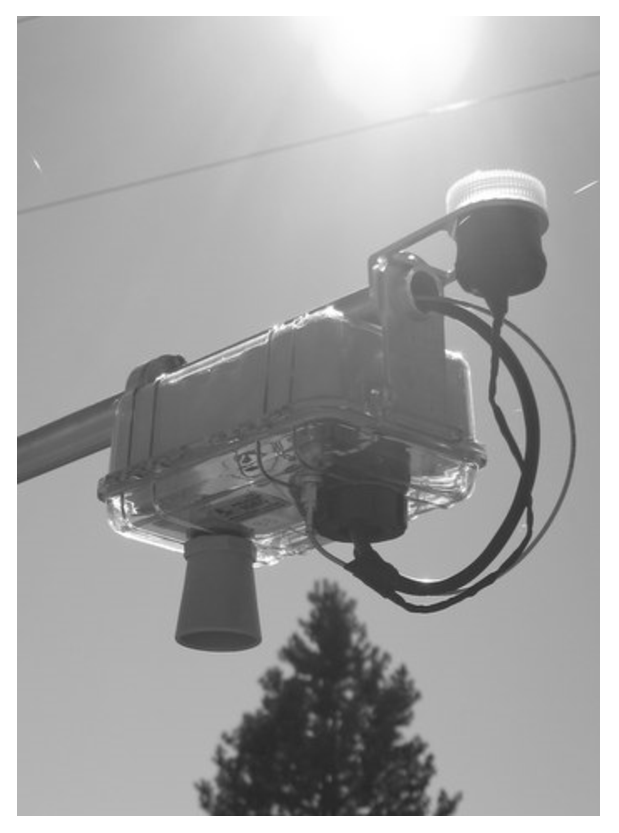
\includegraphics[scale=.50]{brainbox} 
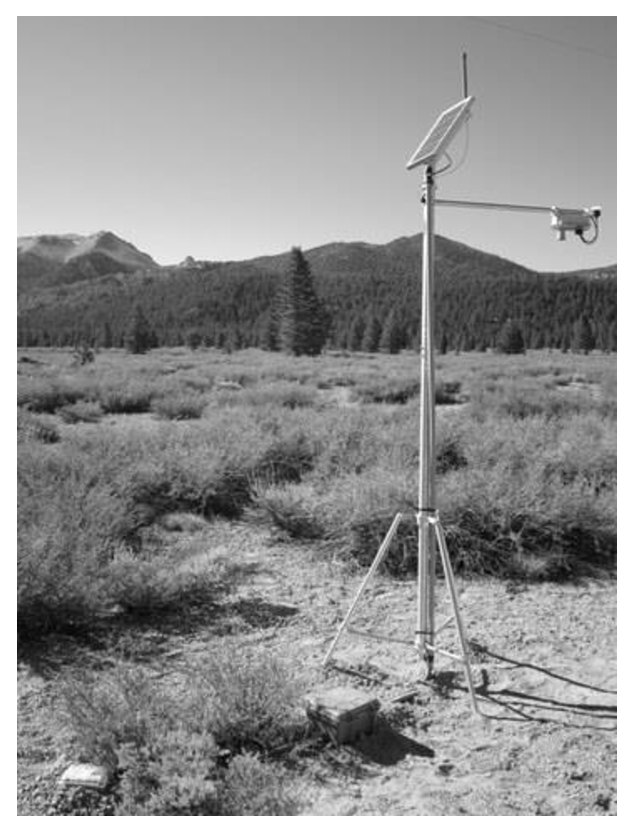
\includegraphics[scale=.50]{tower} 
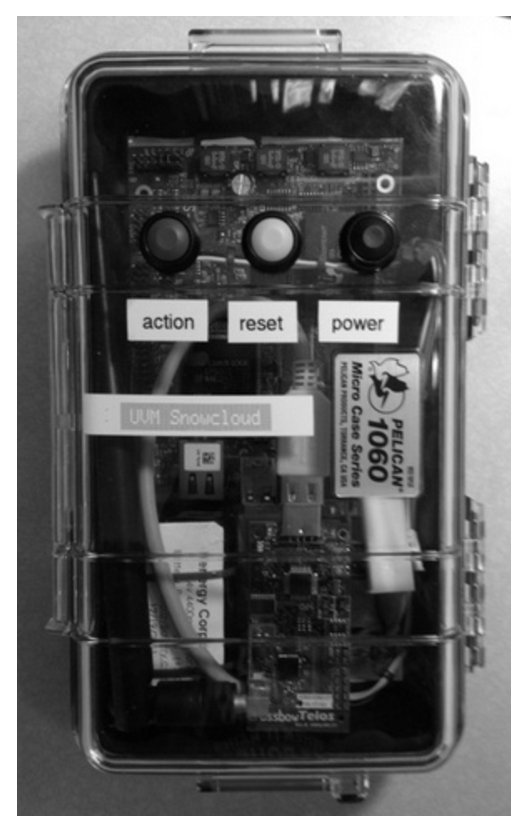
\includegraphics[scale=.50]{harvester} 
\end{center}

\begin{citemize}
\item Distributed data-gathering systems for earth and agricultural sciences.
\item At UVM, focus on alpine snow hydrology.
\begin{citemize}
\item Deployments in California, New Hampshire, Arctic Norway.
\end{citemize}
\end{citemize}
\stopslide

%%%%%

\startslide{Challenges of Programming Sensor Networks}
\begin{citemize}
\item Heavily resource constrained---RAM, ROM, clock cycles, power.
\item e.g., Crossbow TelosB: 4\,MHz, 10\,KiB RAM, 48\,KiB ROM
\item \ldots yet complex, distributed algorithms used
\end{citemize}

State of the art:
\begin{citemize}
\item nesC and TinyOS: optimized for efficiency, widely used.
\item Various \cemph{macroprogramming} proposals, but mostly ad hoc node level programming
  techniques in practice.
\end{citemize}
\stopslide

%%%%%

\startslide{Workflow}
\centering
\scalebox{0.80}{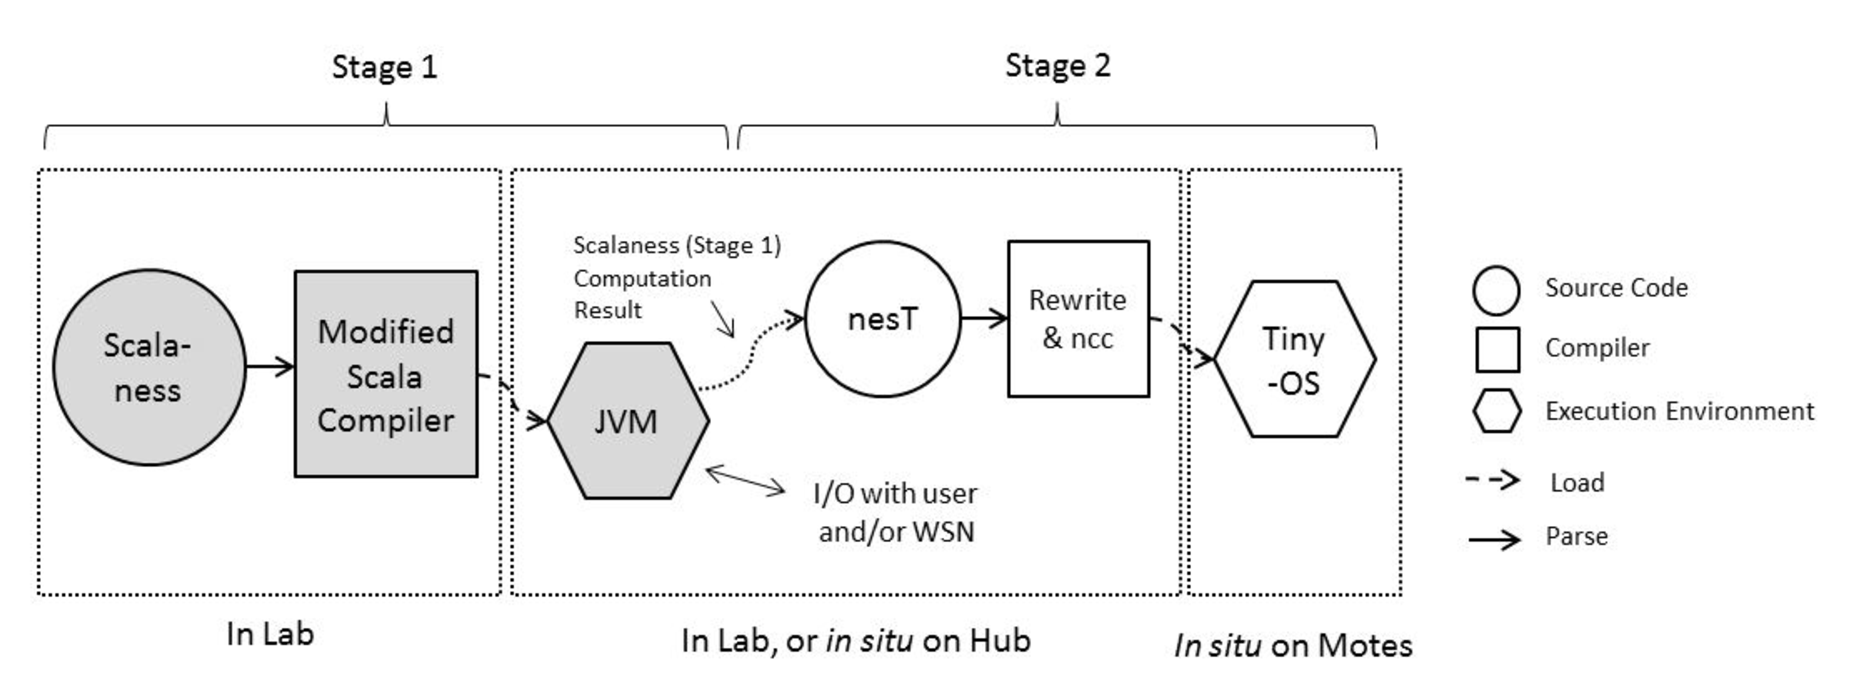
\includegraphics{scalaness}}
\begin{citemize}
\item \cemph{In the lab}: Create first stage program to specialize and compose modules of second
  stage code.
\item \cemph{In the field}: Execute first stage program to generate second stage program
  accounting for field conditions. Deploy to nodes (over the air).
\end{citemize}
\stopslide

%%%%%

\startslide{Our Approach}
\begin{citemize}
\item \cemph{Lightweight macroprogramming}. Scala at metalevel, nesC residuum.
\item Technical features: \cemph{type specialization}, \cemph{process separation}.
\item \cemph{Cross-stage type safety}: type checking at Scala level ensures type safety of nesC
  residuum.
\item \cemph{Well-founded language design}.
\end{citemize}
\stopslide

%%%%%

\startslide{Presentation Outline}
\begin{cenumerate}
\item Motivations, design overview
\item \cemph{Technical details}
\begin{citemize}
\item \cemph{Language design} 
\item Formal foundations
\end{citemize}
\item Language implementation and application
\end{cenumerate}
\stopslide

%%%%%

\startslide{Example: Introducing Some Type Abbreviations}
\lstset{basicstyle=\ttfamily, escapeinside={(*@}{@*)}}
\begin{lstlisting}[language=nesC]
(*@\tt{abbrvt\ mesgT(t) =}@*)
  { src : (*@\tt{t}@*); dest : (*@\tt{t}@*); data : uint8[] };

(*@\tt{abbrvt\ radioT =}@*)
  < at (*@$\subtype$@*) uint >
  { export error_t radio_x((*@\tt{mesgT}@*)(at)*); 
    import error_t handle_radio_r((*@\tt{mesgT}@*)(at)*); };

(*@\tt{abbrvt\ commT =}@*)
  (at (*@$\subtype$@*) uint) (*@$\circ$@*) < >
  { export error_t send((*@\tt{mesgT}@*)(at)*); 
    import error_t handle_receive((*@\tt{mesgT}@*)(at)*); };
\end{lstlisting}
\stopslide

%%%%%

\startslide{Example: nesT Modules}
\lstset{basicstyle=\ttfamily, escapeinside={(*@}{@*)}}
\begin{lstlisting}[language=nesC]
(*@\tt{authSend =}@*)
  < at (*@$\subtype$@*) uint; sendk : uint8[] >  
  { import error_t radio_x((*@\tt{mesgT}@*)(at)*);
    export error_t send(m : (*@\tt{mesgT}@*)(at)*) 
        { radio_x(AES_sign(m, sendk)); }
  };

(*@\tt{authRecv =}@*)
  < at (*@$\subtype$@*) uint; recvk : uint8[] >  
  { import error_t handle_recv((*@\tt{mesgT}@*)(at)*);
    export error_t handle_radio_r(m : (*@\tt{mesgT}@*)(at)*) 
        { if (AES_signed(m, recvk))
              handle_recv(m); }
  };
\end{lstlisting}
\stopslide

%%%%%

\startslide{Example: Scalaness Method}
\lstset{basicstyle=\ttfamily, escapeinside={(*@}{@*)}}
\begin{lstlisting}[language=scalaness]
def authSpecialize
 (nmax   : uint16,
  radioM : radioT,
  keys   : Array[Array[uint8]]) : commT {

    typedef adt (*@$\subtype$@*) uint =
      if (nmax <= 256) uint8 else uint16;

    val sendM = (*@\jinst{authSend}{adt; keys(0)}@*);
    val recvM = (*@\jinst{authRecv}{adt; keys(1)}@*);
    sendM (*@$\ltimes$@*) (*@\jinst{radioM}{adt}@*) (*@$\ltimes$@*) recvM;
}
\end{lstlisting}
\stopslide

%%%%%

\startslide{Example: Generating Residual Program}
\lstset{basicstyle=\ttfamily, escapeinside={(*@}{@*)}}
\begin{lstlisting}[language=scalaness]
val appMR =
  < >
  { export handle_recv(m : (*@\tt{mesgT}@*)(uint8)*) {(*@\ldots@*)} }; 

val appM = 
  < >
  { import send((*@\tt{mesgT}@*)(uint8)*); export main() {(*@\ldots@*)} };  

 image(appM (*@$\ltimes$@*)
         authSpecialize(nmax, radioM, keys) (*@$\ltimes$@*)
           appMR);
\end{lstlisting}
\stopslide

%%%%%

\startslide{Presentation Outline}
\begin{cenumerate}
\item Motivations, design overview
\item \cemph{Technical details}
\begin{citemize}
\item Language design 
\item \cemph{Formal foundations}
\end{citemize}
\item Language implementation and application
\end{cenumerate}
\stopslide

%%%%%

\startslide{\fml\ Foundations} The \fml\ language\footnote{\cref{Yu David Liu, Christian Skalka,
    and Scott Smith. Type-Specialized Staged Programming with Process Separation. Journal of
    Higher Order and Symbolic Computation, 24(4):341-385, 2012.}} was developed to study these
elements at a foundational level.
\begin{citemize}
\item Comprises $F_{\le}$.
\item MetaML-like syntax and semantics, but novel features to moderate interactions between
  separate process spaces.
\item Resricted form of type construction (not full $\lambda_\omega$).
\item Formal metatheory includes cross-stage type safety---residue of partial evaluation of
  well-typed code is guaranteed to be well-typed.
\end{citemize}
\stopslide

%%%%%

\startslide{Sample Scalaness Typing}
$$
\jmodt{\Delta_1}{\margs{\Delta_2, \Gamma}\lc 
  \imports; \exportsty \rc}
$$
Module type form, where:
\begin{citemize}
\item $\Delta_2$, $\Gamma$ type parameter bounds and term parameter types
\item $\imports$, $\exportsty$ import and export type signatures
\item $\Delta_1$ bounds of types constructed externally to the module
\begin{citemize}
\item Early substitution of these types unsound due to possible contravariant use in $\imports;
  \exportsty$.
\end{citemize}
\end{citemize}
$$
\inferrule[ModInstT]
{\Gamma \vdash \tt{e} : \jmodt{\varnothing}{\margs{\vect{t} \subtype \vect{\t}_1; 
 \vect{x} : \vect{\t}_2} \lc \imports; \exportsty \rc} \\
 \Gamma \vdash \ttvec{s} : \jinst{MetaType}{\ttvec{T}_1} \\
 \Gamma \vdash \ttvec{e}_2 : \ttvec{T}_2 \\
 \vdash \codt{\ttvec{T}_1} \subtype \vect{\t}_1 \\
 \vdash \codt{\ttvec{T}_2} \subtype \vect{\t}_2
}
{\Gamma \vdash \jinst{e}{\ttvec{s}; \ttvec{e}_2} : \jmodt{\ttvec{s} \subtype
    \codt{\ttvec{T}_1}}{\margs{} \lc \imports[\ttvec{s}/\vect{t}]; \exportsty[\ttvec{s}/\vect{t}] \rc} }
$$
\stopslide

%%%%%

\startslide{Presentation Outline}
\begin{cenumerate}
\item Motivations, design overview
\item Technical details
\begin{citemize}
\item Language design 
\item Formal foundations
\end{citemize}
\item \cemph{Language implementation and application}
\end{cenumerate}
\stopslide

%%%%%

\startslide{Implementation}
Scalaness/nesT has been implemented.
\begin{citemize}
\item nesT defined as restricted subset of nesC, compiled as nesC with some rewriting
  (e.g.~array bounds checks).
\item Scalaness defined by extension to the Scala compiler.
\item Type checking extends Scala type checker with module types, module operation typings, nesT
  type checking.
\end{citemize}
Web site with samples: \url{http://tinyurl.com/a85z8cu}
\stopslide

%%%%%

\startslide{Application: WSN Session Key Negotiation}
Currently studying authorization schemes for WSNs.
\begin{citemize}
\item WSN may comprise interacting security domains with different credentials and policies.
\item Symmetric keys provide efficient foundation for securing access.
\item Public keys allow symmetric key negotiation (Diffie-Hellman) in ``open world'' model.
\end{citemize}
Public key signature verification wildly expensive in WSNs; around 90 seconds on Crossbow
TelosB.

\cemph{Refactor session key negotiation and authorized access into 
different stages.}
\stopslide

%%%%%

\startslide{Application: WSN Session Key Negotiation}
\hspace*{.6in}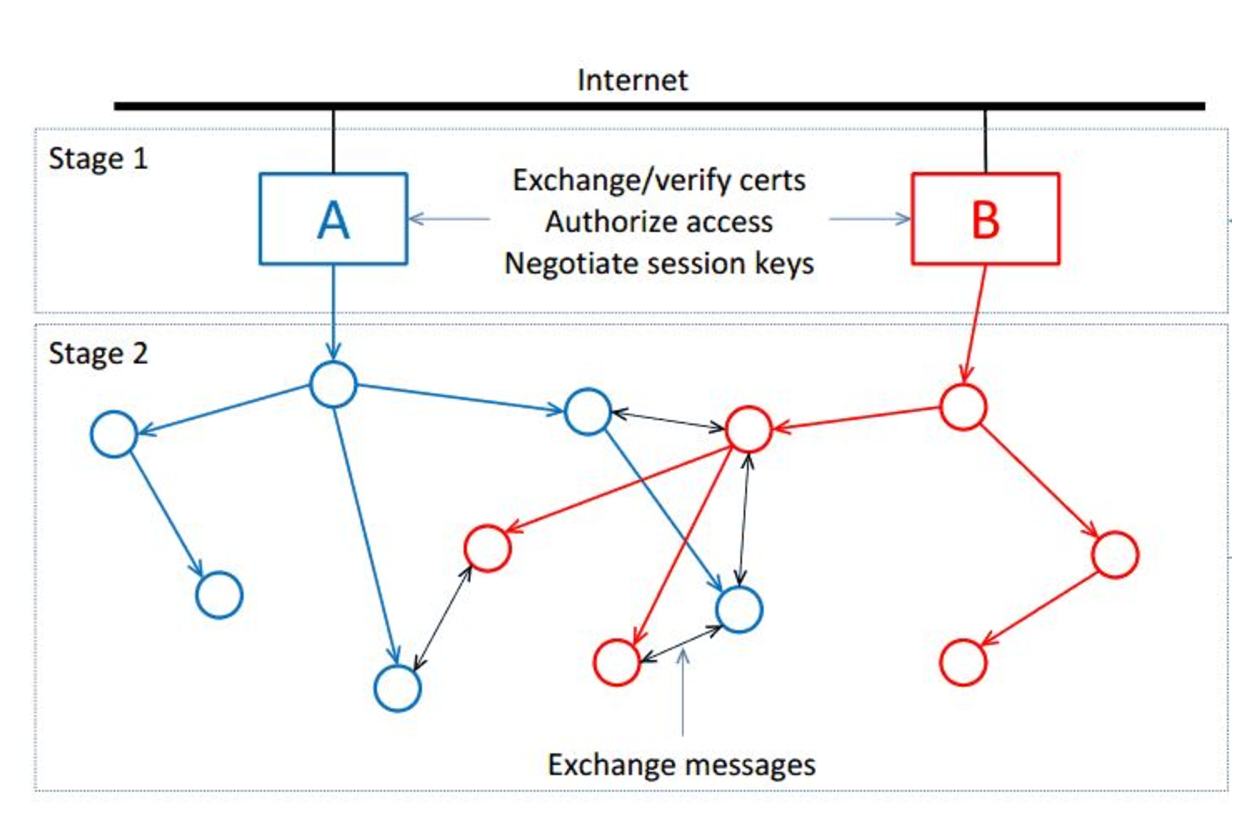
\includegraphics{spartanrpc}

Decreases WSN computational overhead, RAM and ROM consumption. 
\stopslide

%%%%%

\startslide{Results}
\begin{center}
\begin{tabular}{|r||c|c|c|c|} \hline
              & Unsecured & Unstaged* & Staged & Savings\\ \hline
Sensor ROM    &     36254 &    48616 &  36596 & 25\% \\
Sensor RAM    &      2868 &     5417 &   3038 & 44\% \\ \hline
Harvester ROM &     24316 &    35834 &  24436 & 32\% \\
Harvester RAM &      2274 &     4771 &   2402 & 50\% \\ \hline
\end{tabular}
\end{center}
\vspace{1.5in}
{\small * Chapin, Skalka; \textit{SpartanRPC}; Technical Report;
  \url{http://www.cs.uvm.edu/~skalka/skalka-pubs/chapin-skalka-spartanrpctr.pdf}}
\stopslide

%%%%%

\startslide{Future Work}
\begin{citemize}
\item Clarifying ``middle ground'' between language borders.
\item Syntactic transformations; allowing DScalaness syntax in Scalaness programs.
\item Incorporating network communication. 
\item Other applications: backcasting and evolving control.
\end{citemize}
\stopslide

%%%%%

\startslide{Questions?}
\makeatletter
\center{Peter Chapin \textless pchapin@cs.uvm.edu\textgreater}
\center{\cemph{http://tinyurl.com/a85z8cu}}
\makeatother
\stopslide


\end{document}









